\section{Preliminaries}

\begin{frame}{Overfitting in adversarially robust deep learning}
    \begin{itemize}
    % [<+-| alert@+>] % stepwise alerts
        \item One of the surprising characteristics of deep learning is the relative lack of overfitting. 
        \item Deep learning models can often be trained to zero training error without causing any detrimental effects on the generalization performance.
        \item Adversarially robust training has the property that, after a certain point, further training will continue to substantially decrease the robust training loss of the classifier, while increasing the robust test loss (Rice et al., 2020).
        \begin{figure}
            \begin{minipage}[c]{0.55\linewidth}
                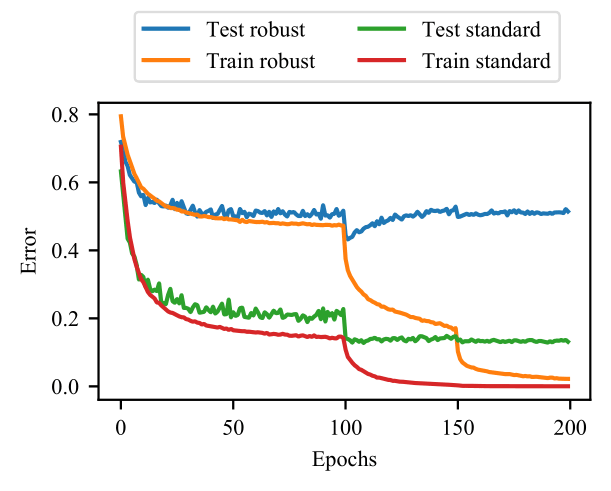
\includegraphics[height=.5\textheight]{pic/cifar10_curve.png}
            \end{minipage}
            \begin{minipage}[c]{0.4\linewidth}
                \caption{The learning curves for a robustly trained model replicating the experiment done by Madry et al. (2017) on CIFAR-10. The curves demonstrate “robust overfitting”; shortly after the first learning rate decay the model momentarily attains $43.2\%$ robust error, and is actually more robust than the model at the end of training, which only attains $51.4\%$ robust test error against a 10-step PGD adversary for $\ell_\infty$ radius of $\epsilon = 8/255$. The learning rate is decayed at 100 and 150 epochs.}\label{fig:cifar10_curve}
            \end{minipage}
        \end{figure}
    \end{itemize}
\end{frame}

\begin{frame}{Overcoming Robust Overfitting}
    \begin{itemize}
    % [<+-| alert@+>] % stepwise alerts
        \item Rice et al. propose to use early stopping as the main contingency against robust overfitting, and demonstrate that it also allows to train models that are more robust than those trained with other regularization techniques (e.g. data augmentation or increased $\ell_2$-regularization).
        \item Other regularization techniques could reduce the impact of overfitting at the cost of producing models that are over-regularized and lack overall robustness and accuracy.
        \item There is one notable exception which is the addition of \emph{external data}.
        \begin{figure}
            \centering
            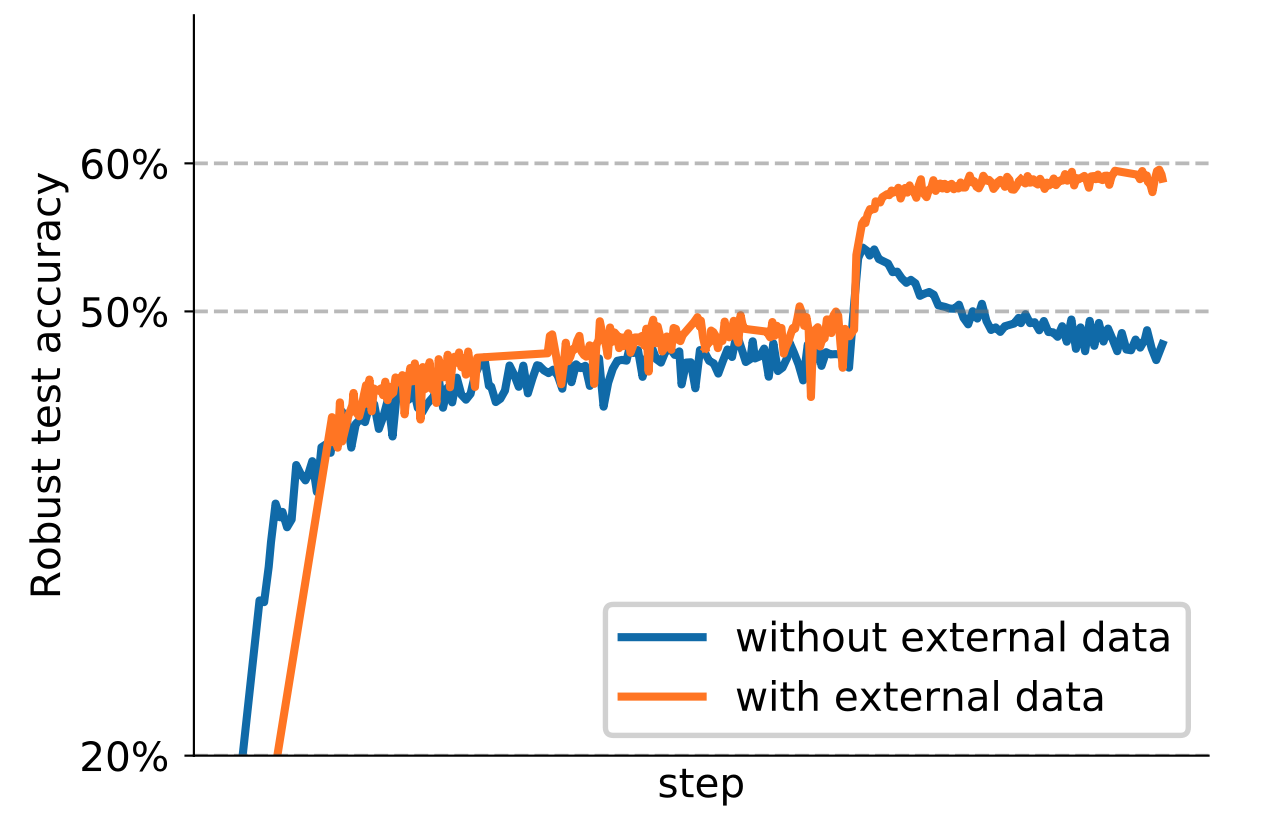
\includegraphics[height=.4\textheight]{pic/external_data.png}
            \caption{Adversarial training with and without additional data from 80M-TI}
            \label{fig:external_data}
        \end{figure}
    \end{itemize}
\end{frame}


\begin{frame}{Averaging Weights Leads to Wider Optima and Better Generalization}
    \begin{itemize}
    % [<+-| alert@+>] % stepwise alerts
        \item Deep neural networks are typically trained by optimizing a loss function with an SGD variant, in conjunction with a decaying learning rate, until convergence.
        \item Simple averaging of multiple points along the trajectory of SGD, with a cyclical or constant learning rate, leads to better generalization than conventional training.
        \item Stochastic Weight Averaging (SWA) procedure finds much flatter solutions than SGD.
        \item In short, SWA is extremely easy to implement, improves generalization, and has almost no computational overhead.
        \item Model weight averaging (WA) can be implemented using an exponential moving average $\mathbf{\theta}'$ of the model parameters $\mathbf{\theta}$ with a decay rate $\tau$: $$\mathbf{\theta}' \leftarrow \tau \cdot \mathbf{\theta}' + (1-\tau)\cdot\mathbf{\theta}$$
        \item WA can significantly improve robustness on a wide range of models and datasets.
    \end{itemize}
\end{frame}

\begin{frame}{Model Weight Averaging}
    \begin{itemize}
    % [<+-| alert@+>] % stepwise alerts
        \item WA leads to a \emph{flatter adversarial loss landscape} and a smaller robust generalization gap.
        \item In addition to improved robustness, WA reduces sensitivity to early stopping. 
        \item However WA is still prone to robust overfitting since the exponential moving average “forgets” older model parameters as training goes on.
        \item We observe that, after the change of learning rate, the averaged weights are increasingly affected by overfitting, thus resulting in worse robust accuracy for the averaged model.
        \begin{figure}
            \centering
            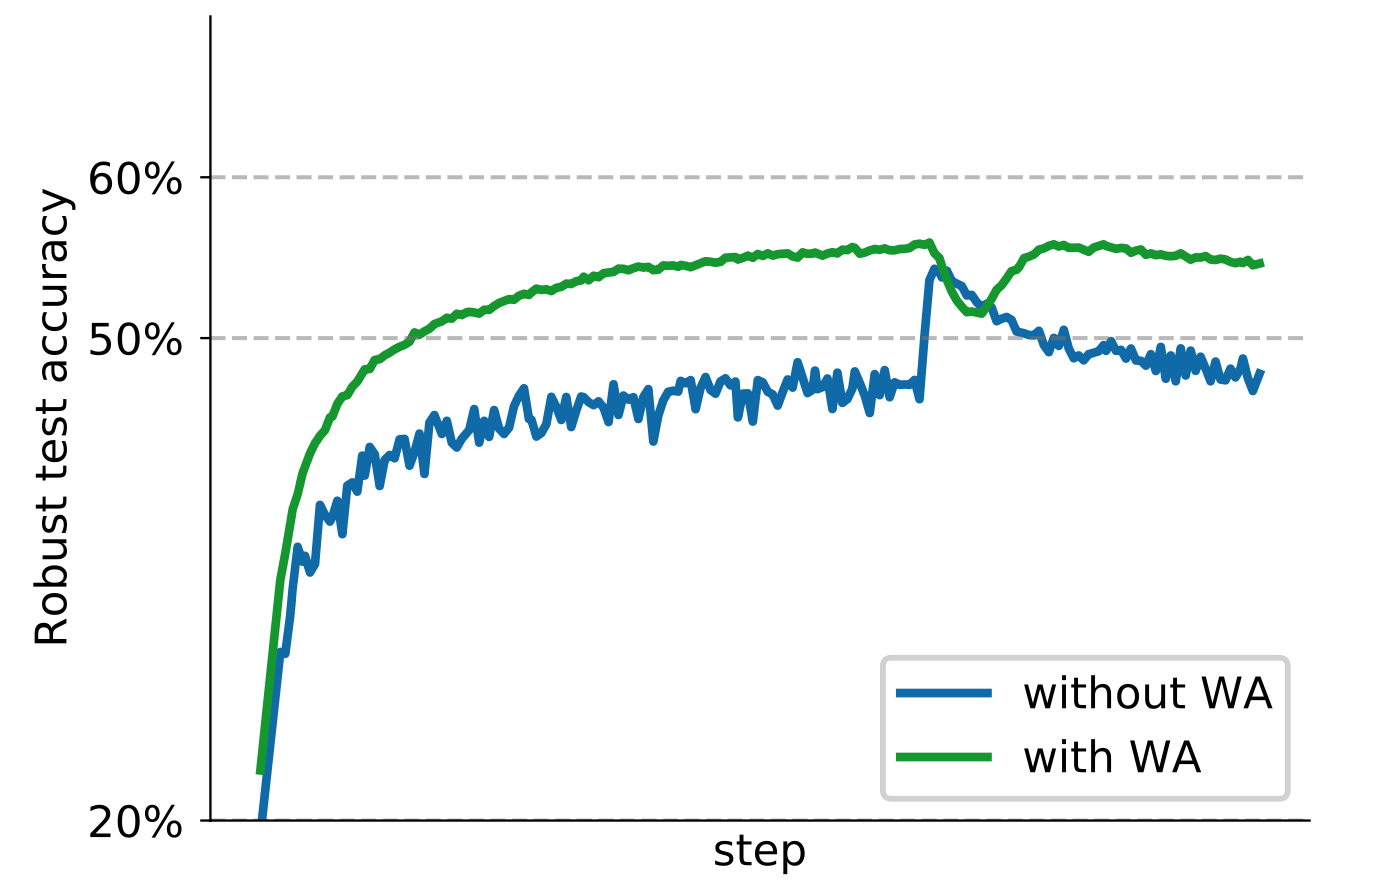
\includegraphics[height=.4\textheight]{pic/weight_averaging.png}
            \caption{Effect of WA without external data}
            \centering
            \label{fig:weight_averaging}
        \end{figure}
    \end{itemize}
\end{frame}

\begin{frame}{Effects of External Data and Weighted Averaging}
    \begin{figure}
        \centering
        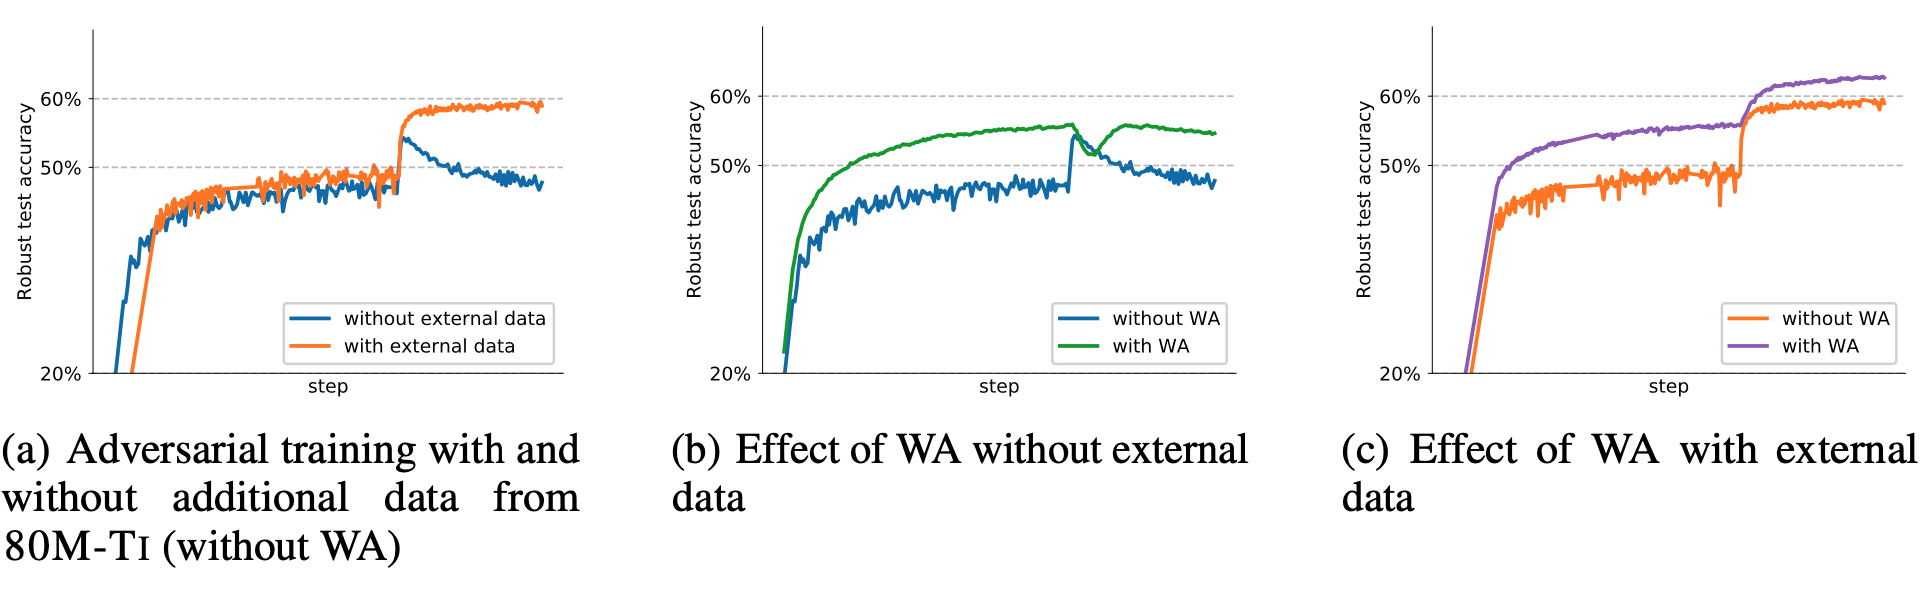
\includegraphics[height=.4\textheight]{pic/ED_WA.png}
        \caption{We compare the robust accuracy against $\epsilon_\infty = 8/255$ on CIFAR-10 of an adversarially trained Wide ResNet (WRN)-28-10. Panel (a) shows the impact of using additional external data from 80M-TI and illustrates robust overfitting. Panel (b) shows the benefit of model weight averaging (WA) despite robust overfitting. Panel (c) shows that WA remains effective and useful even when robust overfitting disappears. The graphs show the evolution of the robust accuracy as training progresses (against $PGD^{40}$). The jump two-thirds through training is due to a drop in learning rate.}
        \label{fig:ED_WA}
    \end{figure}
\end{frame}